\documentclass[letter,11pt]{article}

\usepackage[spanish,es-nodecimaldot]{babel}
\usepackage[utf8]{inputenc}

\usepackage{lmodern}
\usepackage[T1]{fontenc}
\usepackage{textcomp}

\usepackage{framed}
\usepackage[svgnames]{xcolor}
\colorlet{shadecolor}{Gainsboro!50}

\usepackage{enumitem}
\usepackage{graphicx}
\usepackage{pstricks}

\usepackage{anysize}
\marginsize{3cm}{2cm}{2cm}{3cm}

\usepackage{siunitx}
\usepackage{amsmath}
\usepackage{array}
\usepackage{alltt}

\usepackage{fancyhdr}
\usepackage{lastpage}
\pagestyle{fancy}
\fancyhf{}
\fancyhead[LE,RO]{Termodinámica}
\fancyfoot[CO,CE]{\thepage\ de \pageref{LastPage}}

\special{papersize=215.9mm,279.4mm}

\usepackage[
    pdfauthor={Carlos Eduardo Caballero Burgoa},%
    pdftitle={Termodinámica},%
    pdfsubject={Tarea 02},%
    colorlinks,%
    citecolor=black,%
    filecolor=black,%
    linkcolor=black,%
    urlcolor=black,
    breaklinks]{hyperref}
\usepackage{breakurl}

\newcommand{\blankpage}{
\newpage
\thispagestyle{empty}
\mbox{}
\newpage
}

\renewcommand{\arraystretch}{1.2}

\begin{document}

\begin{center}
    {\Large \bf{\underline{Tarea \#02}}}
\end{center}
\vspace{0.1cm}

\begin{enumerate}
\item Considere el cilindro de la figura, en el estado inicial el
cilindro contiene $5[kg]$ de agua saturada a $38^\circ C$. Un embolo con área
transversal de $650[cm^2]$ descansa sobre los topes donde el volumen es de
$30[dm^3]$, la masa del embolo es de $2275[kg]$. Se entrega calor al agua hasta
que el embolo alcanza un volumen de $75[dm^3]$. Para este proceso hallar 2
propiedades en cada estado.

\vspace{0.75cm}
\begin{figure}[!h]
\centering
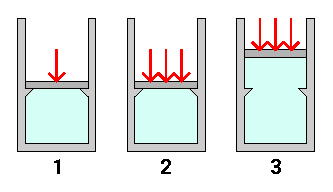
\includegraphics[scale=1.5]{resources/f1.eps}
\end{figure}
\vspace{0.75cm}

\textbf{\underline{Solución}:} \\

\begin{equation*}
    m_A=5[kg]
\end{equation*}
\begin{equation*}
    A_E=650[cm^2]\cdot\frac{1[m]}{100[cm]}\cdot\frac{1[m]}{100[cm]}=0.0650[m^2]
\end{equation*}
\begin{equation*}
    m_E=2275[kg]
\end{equation*}

\underline{Estado 1:} \\

\begin{equation*}
    T_1=38^\circ C
\end{equation*}
\begin{equation*}
    V_1=30[dm^3]\cdot\frac{1[m]}{10[dm]}\cdot\frac{1[m]}{10[dm]}\cdot\frac{1[m]}{10[dm]}=0.03[m^3]
\end{equation*}

Hallamos el volumen especifico:
\begin{equation*}
    v_1=\frac{V_1}{m_A}=\frac{0.03}{5}=0.006[m^3/kg]
\end{equation*}

\underline{Estado 2:} \\

El volumen se mantiene constante:

\begin{equation*}
    v_2=v_1=0.006[m^3/kg]
\end{equation*}

La presión es:

\begin{equation*}
    P_2=\frac{m_E g}{A_E}=\frac{2275[kg]9.8[m/s^2]}{0.0650[m^2]}=343000[Pa]\cdot\frac{1[kPa]}{1000[Pa]}=343[kPa]
\end{equation*}

Según tablas termodinámicas a $350[kPa]$, los valores de saturación son:

\begin{equation*}
    T_{sat}=138.88^\circ C
\end{equation*}
\begin{equation*}
    v_l=0.001079
\end{equation*}
\begin{equation*}
    v_v=0.52425
\end{equation*}

Hallamos el titulo:

\begin{equation*}
    X_2=\frac{v_2-v_l}{v_v-v_l}=\frac{0.006-0.001079}{0.52425-0.001079}=0.009406
\end{equation*}

\underline{Estado 3:} \\

\begin{equation*}
    V_3=75[dm^3]\cdot\frac{1[m]}{10[dm]}\cdot\frac{1[m]}{10[dm]}\cdot\frac{1[m]}{10[dm]}=0.075[m^3]
\end{equation*}

Hallamos el volumen especifico:
\begin{equation*}
    v_3=\frac{V_3}{m_A}=\frac{0.075}{5}=0.015[m^3/kg]
\end{equation*}

La presión se mantiene constante:

\begin{equation*}
    P_3=P_2=343[kPa]
\end{equation*}

Considerando los valores de presión ($350[kPa]$) y temperatura ($138.88^\circ C$), del estado anterior,
calculamos el titulo:

\begin{equation*}
    X_3=\frac{v_3-v_l}{v_v-v_l}=\frac{0.006-0.001079}{0.52425-0.001079}=0.026609
\end{equation*}

Por tanto la temperatura es:

\begin{equation*}
    T_3=T_{sat}=138.88^\circ C
\end{equation*}

\begin{figure}[!h]
\centering
\includegraphics[scale=1.4]{resources/g1.eps}
\end{figure}
\vspace{1.0cm}

\newpage

\item Considere el embolo con su cilindro, dentro el cual se tiene $0.5[kg]$ de
agua a $4[MPa]$ y $400^\circ C$. Se entrega calor al agua hasta que su volumen
aumente en $50\%$ del volumen inicial. Al inicio el resorte NO ejerce ninguna
presión sobre el embolo. La fuerza del resorte se calcula en $F = kx$, donde
$k = 0.9 [kN/cm]$, $x = \text{desplazamiento}$. El diámetro del embolo es
$20 [cm]$. Hallar el volumen final y las 4 propiedades en el estado final.

\vspace{0.75cm}
\begin{figure}[!h]
\centering
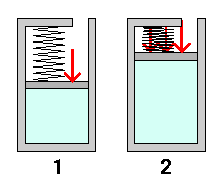
\includegraphics[scale=1.5]{resources/f2.eps}
\end{figure}
\vspace{0.75cm}

\textbf{\underline{Solución}:} \\

\begin{equation*}
    m_A=0.5[kg]
\end{equation*}
\begin{equation*}
    F=kx
\end{equation*}
\begin{equation*}
    k=0.9[\frac{kN}{cm}]\cdot\frac{1000[N]}{1[kN]}\cdot\frac{100[cm]}{1[m]}=90000[N/m]
\end{equation*}
\begin{equation*}
    d_E=20[cm]
\end{equation*}
\begin{equation*}
    r_E=\frac{d_E}{2}=0.1[m]
\end{equation*}

\underline{Estado 1:} \\

\begin{equation*}
    P_1=4000[kPa]
\end{equation*}
\begin{equation*}
    T_1=400^\circ C
\end{equation*}

Hallamos el volumen especifico para $P_1=4000[kPa]$ y $T_1=400^\circ C$ en tablas:

\begin{equation*}
    v_1=0.07341
\end{equation*}

Hallamos el volumen para ese volumen especifico $v_1$:

\begin{equation*}
    v_1=\frac{V_1}{m_A}
\end{equation*}
\begin{equation*}
    V_1=m_A\,v_1=0.5(0.07341)=0.0367[m^3]
\end{equation*}

Según tablas termodinámicas a $4000[kPa]$, los valores de saturación son:

\begin{equation*}
    T_{sat}=250.40^\circ C
\end{equation*}
\begin{equation*}
    v_l=0.001252
\end{equation*}
\begin{equation*}
    v_v=0.04978
\end{equation*}

Hallamos el titulo:

\begin{equation*}
    X_1=\frac{v_1-v_l}{v_v-v_l}=\frac{0.07341-0.001252}{0.04978-0.001252}=1.4869>1
\end{equation*}

\underline{Estado 2:} \\

El volumen es:

\begin{equation*}
    V_2=1.5\,V_1=1.5(0.0367)=0.055[m^3]
\end{equation*}

El volumen especifico es:

\begin{equation*}
    v_2=1.5\,v_1=1.5(0.07341)=0.1101
\end{equation*}

La presión es la suma de la presión anterior y la presión ejercida por el resorte:

\begin{equation*}
    P_2=P_1+P_R
\end{equation*}

La presión ejercida por el resorte es:

\begin{equation*}
    P_R=\frac{F_R}{A}=\frac{kx}{\pi r^2}
\end{equation*}

Considerando el volumen de un cilindro, despejamos $x$:

\begin{equation*}
    \Delta V=\pi r^2 x
\end{equation*}
\begin{equation*}
    x=\frac{\Delta V}{\pi r^2}=\frac{V_2-V_1}{\pi r^2}
\end{equation*}

Por tanto:

\begin{equation*}
    P_R=\frac{k}{\pi r^2}\frac{V_2-V_1}{\pi r^2}=k\frac{V_2-V_1}{\pi^2 r^4}=1673.5[kPa]
\end{equation*}
\begin{equation*}
    P_2=P_1+P_R=5673.5[kPa]
\end{equation*}

Hallamos la temperatura a partir de la presión ($P=6000[kPa]$) y el volumen especifico ($v=0.11321$) en las tablas termodinámicas:

\begin{equation*}
    T_2=1200^\circ C
\end{equation*}

\begin{figure}[!h]
\centering
\includegraphics[scale=1.5]{resources/g2.eps}
\end{figure}
\vspace{1.0cm}

\newpage

\item Dentro un cilindro con su embolo se tiene $2[kg]$ de agua saturada, con un
titulo del $25\%$. La masa del embolo es $40[kg]$ y su diámetro $10[cm]$, la
presión atmosférica es $1.3[kgf/cm^2]$. Además sobre el embolo hay un peso que
ejerce una presión de $120[kPa]$. Se entrega calor al sistema hasta que su
presión sea de $0.7[MPa]$. Hallar 2 propiedades termodinámicas en cada estado.
El volumen en los topes es el doble del volumen inicial.

\vspace{0.75cm}
\begin{figure}[!h]
\centering
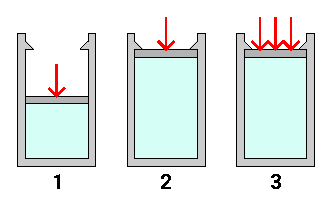
\includegraphics[scale=1.3]{resources/f3.eps}
\end{figure}
\vspace{0.75cm}

\textbf{\underline{Solución}:} \\

\begin{equation*}
    m_A=2[kg]
\end{equation*}
\begin{equation*}
    m_E=40[kg]
\end{equation*}
\begin{equation*}
    d_E=10[cm]
\end{equation*}
\begin{equation*}
    r_E=\frac{d_E}{2}=0.05[m]
\end{equation*}
\begin{equation*}
    P_{atm}=1.3[\frac{kgf}{cm^2}]\cdot\frac{100[cm]}{1[m]}\cdot\frac{100[cm]}{1[m]}\cdot\frac{9.8[N]}{1[kgf]}\cdot\frac{1[kPa]}{1000[Pa]}=127.4[kPa]
\end{equation*}
\begin{equation*}
    P_{extra}=120[kPa]
\end{equation*}

\underline{Estado 1:} \\

\begin{equation*}
    X_1=0.25
\end{equation*}

La presión es la suma de las presiones atmosférica, del embolo y el peso adicional:

\begin{equation*}
    P_1=P_{atm}+P_E+P_{extra}
\end{equation*}

Donde la presión ejercida por el embolo es:

\begin{equation*}
    P_E=\frac{m_E\,g}{A_E}=\frac{m_E\,g}{\pi r^2}=\frac{40(9.8)}{\pi(0.05)^2}=49.911[kPa]
\end{equation*}

Por tanto la presión ($P_1$) es:

\begin{equation*}
    P_1=P_{atm}+P_E+P_{extra}=127.4+49.911+120=297.31[kPa]
\end{equation*}

Según tablas termodinámicas a $300[kPa]$, los valores de saturación son:

\begin{equation*}
    T_{sat}=133.55^\circ C
\end{equation*}
\begin{equation*}
    v_l=0.001073
\end{equation*}
\begin{equation*}
    v_v=0.60582
\end{equation*}

Hallamos el volumen especifico:

\begin{equation*}
    v_1 = v_l + X(v_v-v_l)= 0.001073+0.25(0.60582-0.001073)=0.1522[m^3/kg]
\end{equation*}

\underline{Estado 2:} \\

El volumen se duplica:

\begin{equation*}
    V_2=2\,V_1
\end{equation*}
\begin{equation*}
    v_2=2\,v_1=2(0.1522)=0.3045[m^3/kg]
\end{equation*}

La presión se mantiene constante:

\begin{equation*}
    P_2=P_1
\end{equation*}

Por tanto los valores de saturación no varían respecto al estado anterior:

\begin{equation*}
    T_{sat}=133.55^\circ C
\end{equation*}
\begin{equation*}
    v_l=0.001073
\end{equation*}
\begin{equation*}
    v_v=0.60582
\end{equation*}

Hallamos el titulo:

\begin{equation*}
    X_2=\frac{v_2-v_l}{v_v-v_l}=\frac{0.3045-0.001073}{0.60582-0.001073}=0.5016
\end{equation*}

\underline{Estado 3:} \\

El volumen es constante:

\begin{equation*}
    V_3=V_2
\end{equation*}
\begin{equation*}
    v_3=v_2
\end{equation*}

La presión se incrementa:

\begin{equation*}
    P_3=700[kPa]
\end{equation*}

Según tablas termodinámicas a $700[kPa]$, los valores de saturación son:

\begin{equation*}
    T_{sat}=164.97^\circ C
\end{equation*}
\begin{equation*}
    v_l=0.001108
\end{equation*}
\begin{equation*}
    v_v=0.27286
\end{equation*}

Hallamos el titulo:

\begin{equation*}
    X_3=\frac{v_3-v_l}{v_v-v_l}=\frac{0.3045-0.001108}{0.27286-0.001108}=1.1165>1
\end{equation*}

Hallamos la temperatura a partir de la presión ($P=800[kPa]$) y el volumen especifico ($v=0.29314$) en las tablas termodinámicas:

\begin{equation*}
    T_3=250^\circ C
\end{equation*}

\begin{figure}[!h]
\centering
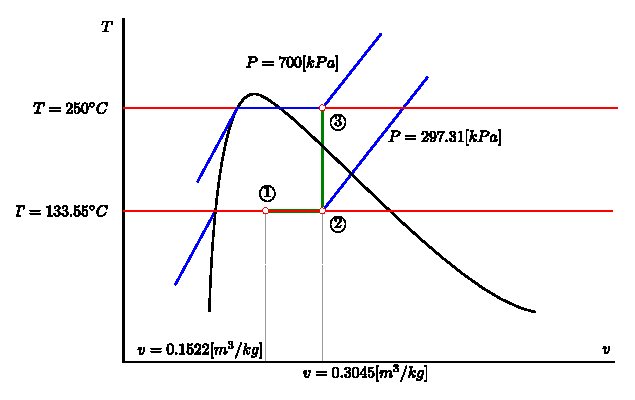
\includegraphics[scale=1.5]{resources/g3.eps}
\end{figure}
\vspace{1.0cm}

\newpage

\item Dentro un cilindro con su embolo se tiene $1[kg]$ de agua a $20^\circ C$
con $0.1[m^3]$ de volumen. Inicialmente el pistón descansa sobre los topes, para
elevarlo al pistón se requiere una presión del agua de $400[kPa]$. ¿Qué
temperatura alcanza el agua cuando el embolo empieza a elevarse después del
calentamiento? Si el calentamiento continua hasta que el agua esta como vapor
saturado, hallar la temperatura final.

\vspace{0.75cm}
\begin{figure}[!h]
\centering
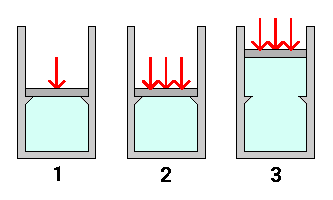
\includegraphics[scale=1.5]{resources/f4.eps}
\end{figure}
\vspace{0.75cm}

\textbf{\underline{Solución}:} \\

\begin{equation*}
    m_A=1[kg]
\end{equation*}

\underline{Estado 1:} \\

\begin{equation*}
    T_1=20^\circ C
\end{equation*}
\begin{equation*}
    V_1=0.1[m^3]
\end{equation*}

Por tanto el volumen especifico es:

\begin{equation*}
    v_1=\frac{V_1}{m_A}=\frac{0.1}{1}=0.1[m^3/kg]
\end{equation*}

\underline{Estado 2:} \\

\begin{equation*}
    P_2=400[kPa]
\end{equation*}

El volumen se mantiene constante:

\begin{equation*}
    v_2=v_1=0.1[m^3/kg]
\end{equation*}

Según tablas termodinámicas a $400[kPa]$, los valores de saturación son:

\begin{equation*}
    T_{sat}=143.63^\circ C
\end{equation*}
\begin{equation*}
    v_l=0.001084
\end{equation*}
\begin{equation*}
    v_v=0.46246
\end{equation*}

Hallamos el titulo:

\begin{equation*}
    X_2=\frac{v_2-v_l}{v_v-v_l}=\frac{0.1-0.001084}{0.46246-0.001084}=0.2144
\end{equation*}

\underline{Estado 3:} \\

Cuando toda el agua se ha convertido en vapor ($X_3=1$), el volumen especifico es:

\begin{equation*}
    v_3=v_v=0.46246
\end{equation*}

La presión se mantiene constante, y la temperatura es la temperatura de saturación:

\begin{equation*}
    P_3=P_2=400[kPa]
\end{equation*}
\begin{equation*}
    T_3=T_{sat}=143.63^\circ C
\end{equation*}

\begin{figure}[!h]
\centering
\includegraphics[scale=1.5]{resources/g4.eps}
\end{figure}
\vspace{1.0cm}

\end{enumerate}

\end{document}

